\documentclass{article} % For LaTeX2e
\usepackage{nips13submit_e,times}
\usepackage{hyperref}
\usepackage{url}
\usepackage[dvips]{graphicx}
%\documentstyle[nips13submit_09,times,art10]{article} % For LaTeX 2.09
\usepackage{amssymb,amsmath,mathrsfs}
\usepackage[russian,english]{babel}
\usepackage{algorithm}
\usepackage[noend]{algorithmic}
\usepackage{multicol}
\usepackage{subfig}
\graphicspath{{./eps//}}
\captionsetup{belowskip=4pt,aboveskip=4pt}

\def\algorithmicrequire{\textbf{Input:}}
\def\algorithmicensure{\textbf{Output:}}
\def\algorithmicif{\textbf{if}}
\def\algorithmicthen{\textbf{then}}
\def\algorithmicelse{\textbf{else}}
\def\algorithmicelsif{\textbf{else if}}
\def\algorithmicfor{\textbf{for}}
\def\algorithmicforall{\textbf{for all}}
\def\algorithmicdo{}
\def\algorithmicwhile{\textbf{while}}
\def\algorithmicrepeat{\textbf{repeat}}
\def\algorithmicuntil{\textbf{until}}
\def\algorithmicloop{\textbf{loop}}
\def\algorithmicgoto{\textbf{goto step}}
\def\algorithmicreturn{\textbf{return}}
\newcommand{\LINEIF}[2]{%
    \STATE\algorithmicif\ {#1}\ \algorithmicthen\ {#2} %
}
\newcommand{\GOTO}[1]{%
    \algorithmicgoto\ {\ref{#1};} %
}

\def\AA{A}
\def\XX{\mathbb{X}}
\def\RR{\mathbb{R}}
\def\HH{\mathbb{H}}
\def\LR{\text{LR}}
\newcommand{\X}{\bar X}
\newcommand{\XXell}{[\XX]^\ell}
\def\CC_#1^#2{\tbinom{#1}{#2}}
\def\eps{\epsilon}
\newcommand{\Arg}{\mathop{\rm Arg}\limits}
\newcommand{\sign}{\mathop{\rm sign}\limits}
\providecommand{\Prob}{\mathsf{P}}
\def\Prbig[#1]{\Prob\bigl[#1\bigr]}
\def\PrBig[#1]{\Prob\Bigl[#1\Bigr]}
\newcommand{\Expect}{\mathsf{E}}
\newcommand{\eqdef}{\equiv}

\newcommand{\hypergeom}[5]{{#1}_{#2}^{#4,\:#3}\left(#5\right)}
\newcommand{\hyper}[4]{\hypergeom{h}{#1}{#2}{#3}{#4}}
\newcommand{\Hyper}[4]{\hypergeom{H}{#1}{#2}{#3}{#4}}
\newcommand{\HyperR}[4]{\hypergeom{\bar{H}}{#1}{#2}{#3}{#4}}

\newtheorem{theorem}{Theorem}
\newtheorem{lemma}[theorem]{Lemma}
\newtheorem{definition}[theorem]{Definition}
\newtheorem{claim}[theorem]{Claim}
\newtheorem{corollary}[theorem]{Corollary}
\newcommand{\qed}{\hfill\rule{7pt}{7pt}}
\newenvironment{proof}{\noindent{\bf Proof:}}{\qed\medskip}

\title{Computable combinatorial overfitting bounds}

\author{
Konstantin Vorontsov \\
Dorodnitsyn Computing Centre, Russian Academy of Sciences \\
\texttt{voron@forecsys.ru} \\
\And
Alexander Frey \\
Moscow Institute of Physics and Technology \\
\texttt{sashafrey@gmail.com} \\
\And
Evgeny Sokolov \\
Moscow State University \\
\texttt{sokolov.evg@gmail.com} \\
}

% The \author macro works with any number of authors. There are two commands
% used to separate the names and addresses of multiple authors: \And and \AND.
%
% Using \And between authors leaves it to \LaTeX{} to determine where to break
% the lines. Using \AND forces a linebreak at that point. So, if \LaTeX{}
% puts 3 of 4 authors names on the first line, and the last on the second
% line, try using \AND instead of \And before the third author name.

\newcommand{\fix}{\marginpar{FIX}}
\newcommand{\new}{\marginpar{NEW}}

%\nipsfinalcopy % Uncomment for camera-ready version

\begin{document}
\English

\section*{Appendix}
\newcommand{\wtil}{\widetilde}
\def\XYtext(#1,#2)#3{\rlap{\kern#1\lower-#2\hbox{#3}}}


\begin{theorem}[FC-bound]
\label{thOneAlg}
    For any set $\XX$,
    any $\eps\in [0,1]$,
    and a~fixed classifier~$a$ such that ${m=n(a,\XX)}$
    the probability of~overfitting is~given by the left tail of the hypergeometric distribution:
    \begin{equation}
    \label{eq:OCbound}
        Q_\eps(a, \XX)
        %\Prbig[ \delta(a,X) \geq \eps ]
        =
        \Hyper{L}{m}{\ell}{ \tfrac{\ell}{L} (m-\eps k) }.
    \end{equation}
\end{theorem}
\begin{proof}
    Denote ${s=n(a,X)}$ and rewrite the overfitting condition
    ${\delta(a,X) \geq \eps}$
    as
    $\tfrac1k (m-s) - \tfrac{1}{\ell} s \geq \eps$
    or equivalently
    ${s \leq \tfrac{\ell}{L} (m-\eps k) \eqdef s_m(\eps) }$. Then
    \[
        Q_\eps
        =
        \Prob\bigl[
            n(a,X) \!\leq\! s_m(\eps)
        \bigr]
        =
        \sum\limits_{s=s_0}^{\lfloor s_m(\eps) \rfloor}
        \Prob\bigl[
            n(a,X) \!=\! s
        \bigr]
        =
        \sum\limits_{s=s_0}^{\lfloor s_m(\eps) \rfloor}
        \hyper{L}{m}{\ell}{s}
        =
        \Hyper{L}{m}{\ell}{ s_m(\eps) }.
    \]
    \vskip-3ex
\end{proof}

\begin{theorem}[VC-bound]
\label{thOneAlg}
    For any set $\XX$,
    any learning algorithm~$\mu$,
    and any $\eps\in [0,1]$
    the probability of~large uniform deviation is bounded by the sum of FC-bounds over the set~$A$:
    \begin{equation}
    \label{eq:VCbound}
        %Q_\eps(\mu, \XX)
        \wtil Q_\eps(A, \XX)
        %\Prbig[ \delta(a,X) \geq \eps ]
        \leq
        \sum_{a\in A}
        \Hyper{L}{m}{\ell}{ \tfrac{\ell}{L} (m-\eps k) },
        \quad
        m = n(a,\XX).
    \end{equation}
\end{theorem}
\begin{proof}
    %Apply a union bound which is in fact a substitute of binary values sum for their maximum:
     Apply a union bound substituting the maximum of binary values by their sum:
    \[
        \wtil Q_{\eps} =
        \Prob
        \max_{a\in A}
        \bigl[
            \delta(a,X) \!\geq\! \eps
        \bigr]
        \leq
        \sum_{a\in A}
        \Prob
        \bigl[
            \delta(a,X) \!\geq\! \eps
        \bigr]
        =
        \sum_{a\in A}
        \Hyper{L}{m}{\ell}{s_m(\eps)},
        \quad
        m = n(a).
    \]
    \vskip-3ex
\end{proof}

Further weakening gives a~well known form of the VC-bound:
\[
    \wtil Q_\eps(A, \XX)
    \leq
    |A| \max_m \Hyper{L}{m}{\ell}{s_m(\eps)}
    \leq
    |A| \cdot \tfrac32 e^{-\eps^2\ell},
    \quad
    \text{if } \ell=k,
\]
where $|A|$ is~called a \emph{shattering coefficient} of~the set of classifiers~$A$ on~the~set~$\XX$.

\subsection*{The principle of protective and prohibitive subsets}
\label{sec:ProtProh}

The principle of protective and prohibitive sets~\cite{voron10pria-eng}
is based on the conjecture that
the necessary and sufficient condition for $\mu X=a$ can be specified explicitly
for any classifier $a\in A$
in~terms of subsets of~objects.
From this conjecture an exact $Q_\eps$ bound has been derived.

In~this work we use a similar conjecture relaxed to the necessary condition
and derive an upper bound which has a~simpler form.

\begin{theorem}
\label{hyp:1}
    For each classifier $a\in A$  there exists
    a~\emph{protective subset} $X_a\in \XX$ and
    a~\emph{prohibitive subset} $X'_a\in \XX$ such that
    for any $X\in\XXell$
    \begin{equation}
    \label{eq:hyp1}
    	\bigl[ \mu X \!=\! a \bigr] \leq
        \bigl[X_a \!\subseteq\! X \bigr]
        \bigl[X'_a \!\subseteq\! \X \bigr].
    \end{equation}
\end{theorem}

The subset $\XX{\setminus} X_a{\setminus} X'_a$
is~called \emph{neutral} for a~classifier~$a$.
The presence or absence of neutral objects in a~training sample~$X$
does not change the result of learning~$\mu X$.
Later we will give nontrivial examples of $\mu$ and $A$ that satisfy conjecture~\ref{hyp:1}.

\begin{lemma}
\label{lem1}
    If conjecture~\ref{hyp:1} holds,
    then the probability to~learn a~classifier~$a$ can be bounded:
    \[
        \Prbig[ \mu X\!=\!a ]
        \leq
        P_a
        \equiv
        {\CC_{L_a}^{\ell_a}} / {\CC_{L}^{\ell}},
    \]
    where
    $L_a = L - |X_a| - |X'_a|$ and
    $\ell_a = \ell - |X_a|$
    are the number of neutral objects for~a~classifier~$a$ in the general set~$\XX$ and sample~$X$ respectively.
\end{lemma}
\begin{proof}
    According to the conjecture
    ${
        \Prbig[ \mu X\!=\!a ]
        \leq
        \Prob
        \bigl[  X_a\subseteq  X \bigr]
        \bigl[ X'_a\subseteq \X \bigr]
    }$.
    The right-hand side
    is a fraction of~partitions ${\XX=X\sqcup\X}$ such that
    ${X_a\subseteq  X}$ and ${X'_a\subseteq  \X}$.
    The number of~such partitions is equal to~$\CC_{L_a}^{\ell_a}$.
    The number of all partitions is equal to~$\CC_{L}^{\ell}$,
    hence their ratio gives~$P_a$.
\end{proof}

\begin{theorem}
\label{th:1}
    If conjecture~\ref{hyp:1} holds, then
    for any $\eps\in[0,1]$
    the bound on probability of overfitting is
    \begin{equation}
    \label{eq:th1}
        Q_\eps
        \leq
        \sum_{a\in \AA} P_a \Hyper{L_a}{m_a}{\ell_a}{s_a(\eps)},
    \end{equation}
    where
    ${m_a = n(a,\XX{\setminus} X_a {\setminus} X'_a)}$
    is a~number of errors that classifier~$a$ produces on~neutral objects and
    ${s_a(\eps) = \tfrac\ell L \bigl( n(a)-\eps k \bigr) - n(a,X_a)}$
    is a~largest number of errors $n(a,X{\setminus}X_a)$
    that classifier~$a$ produces on~neutral training objects
    provided that discrepancy $\delta(a,X)$ exceeds~$\eps$.
\end{theorem}

\begin{proof}
    The probability of~overfitting~$Q_\eps$
    can be found as a total probability
    from probability to~learn each of classifiers $\Prbig[ \mu X\!=\!a ]$
    and conditional probabilities
    ${
        Q_{\eps|a} = \Prbig[ \delta(a,X) \!\geq\! \eps \mid a\!=\!\mu X ]
    }$:
    \[
        Q_\eps
        =
        \sum_{a\in \AA}
            \Prbig[ \mu X\!=\!a ] Q_{\eps|a}
        \leq
        \sum_{a\in \AA}
            P_a Q_{\eps|a}.
    \]
    The conditional probability $Q_{\eps|a}$ can be obtained from theorem~\ref{thOneAlg}
    by~taking into account that
    the subsets $X_a$ and $X'_a$ can not be involved in~partitioning given a~fixed classifier~$a$.
    Only $L_a$~neutral objects are partitioned
    into $\ell_a$~training and $L_a-\ell_a$ testing objects.
    To~employ theorem~\ref{thOneAlg} we~express the discrepancy $\delta(a,X)$
    in~terms or the number of errors on neutral training objects $s = n(a,X{\setminus} X_a)$:
    \[
        \delta(a,X) =
        \tfrac1k \bigl( n(a)-s-n(a,X_a) \bigr) -
        \tfrac1\ell \bigl( s+n(a,X_a) \bigr).
    \]
    Condition $\delta(a,X)\geq \eps$ is~equivalent to $s\leq s_a(\eps)$.
    Then $Q_{\eps|a} = \Hyper{L_a}{m_a}{\ell_a}{ s_a(\eps) }$
    and~\eqref{eq:th1} holds.
\end{proof}

Note that the sum $\sum_a P_a$ can be interpreted
as a~degree of looseness of the bound~\eqref{eq:th1}.
The~bound is~exact if this sum is equal to~1.


\subsection*{The splitting and connectivity graph}
Define an order relation on classifiers $a\leq b$ as a natural order over their error vectors:
$a_i \leq b_i$ for all $i=1,\ldots,L$.
Define a~metric on classifiers as a Hamming distance between error vectors:
$\rho(a,b) = \sum_{i=1}^L |a_i-b_i|$.
Classifiers $a$ and $b$ are called \emph{connected} if $\rho(a,b) = 1$.
Define the precedence relation on classifiers $a\prec b$ as
$\bigl(a\leq b\bigr) \wedge \bigl( \rho(a,b)=1 \bigr)$.

%\bigskip
%{\LARGE
%$x_1$ $x_2$ $x_3$ $x_4$ $x_5$ $x_6$ $x_7$ $x_8$ $x_9$ $x_{10}$ }
%\bigskip

The set of classifiers $A$ can be represented by
a~multipartite directed graph $\langle A, E \rangle$
that we call the \emph{splitting and connectivity graph} (SC-graph)
in which vertices are classifiers, and
edges $(a,b)$ are pairs of classifiers such that $a\prec b$,
see example on~Figure~\ref{fig:SC-graph-lin}.
The partite subsets $A_m = \{ a\in A\colon n(a)=m \}$
are called \emph{error layers}, $m=0,\ldots,L$.
Each edge of the SC-graph $(a,b)$ corresponds to an object $x_{ab}\in\XX$
such that $I(a,x_{ab})=0$ and $I(b,x_{ab})=1$.

\begin{figure}[t]
    \noindent\centering
    \raisebox{3mm}{(a)~}
    \includegraphics[width = 55mm]{SimpleSample1num.PNG.eps}
    \qquad
    \raisebox{3mm}{(b)~}
    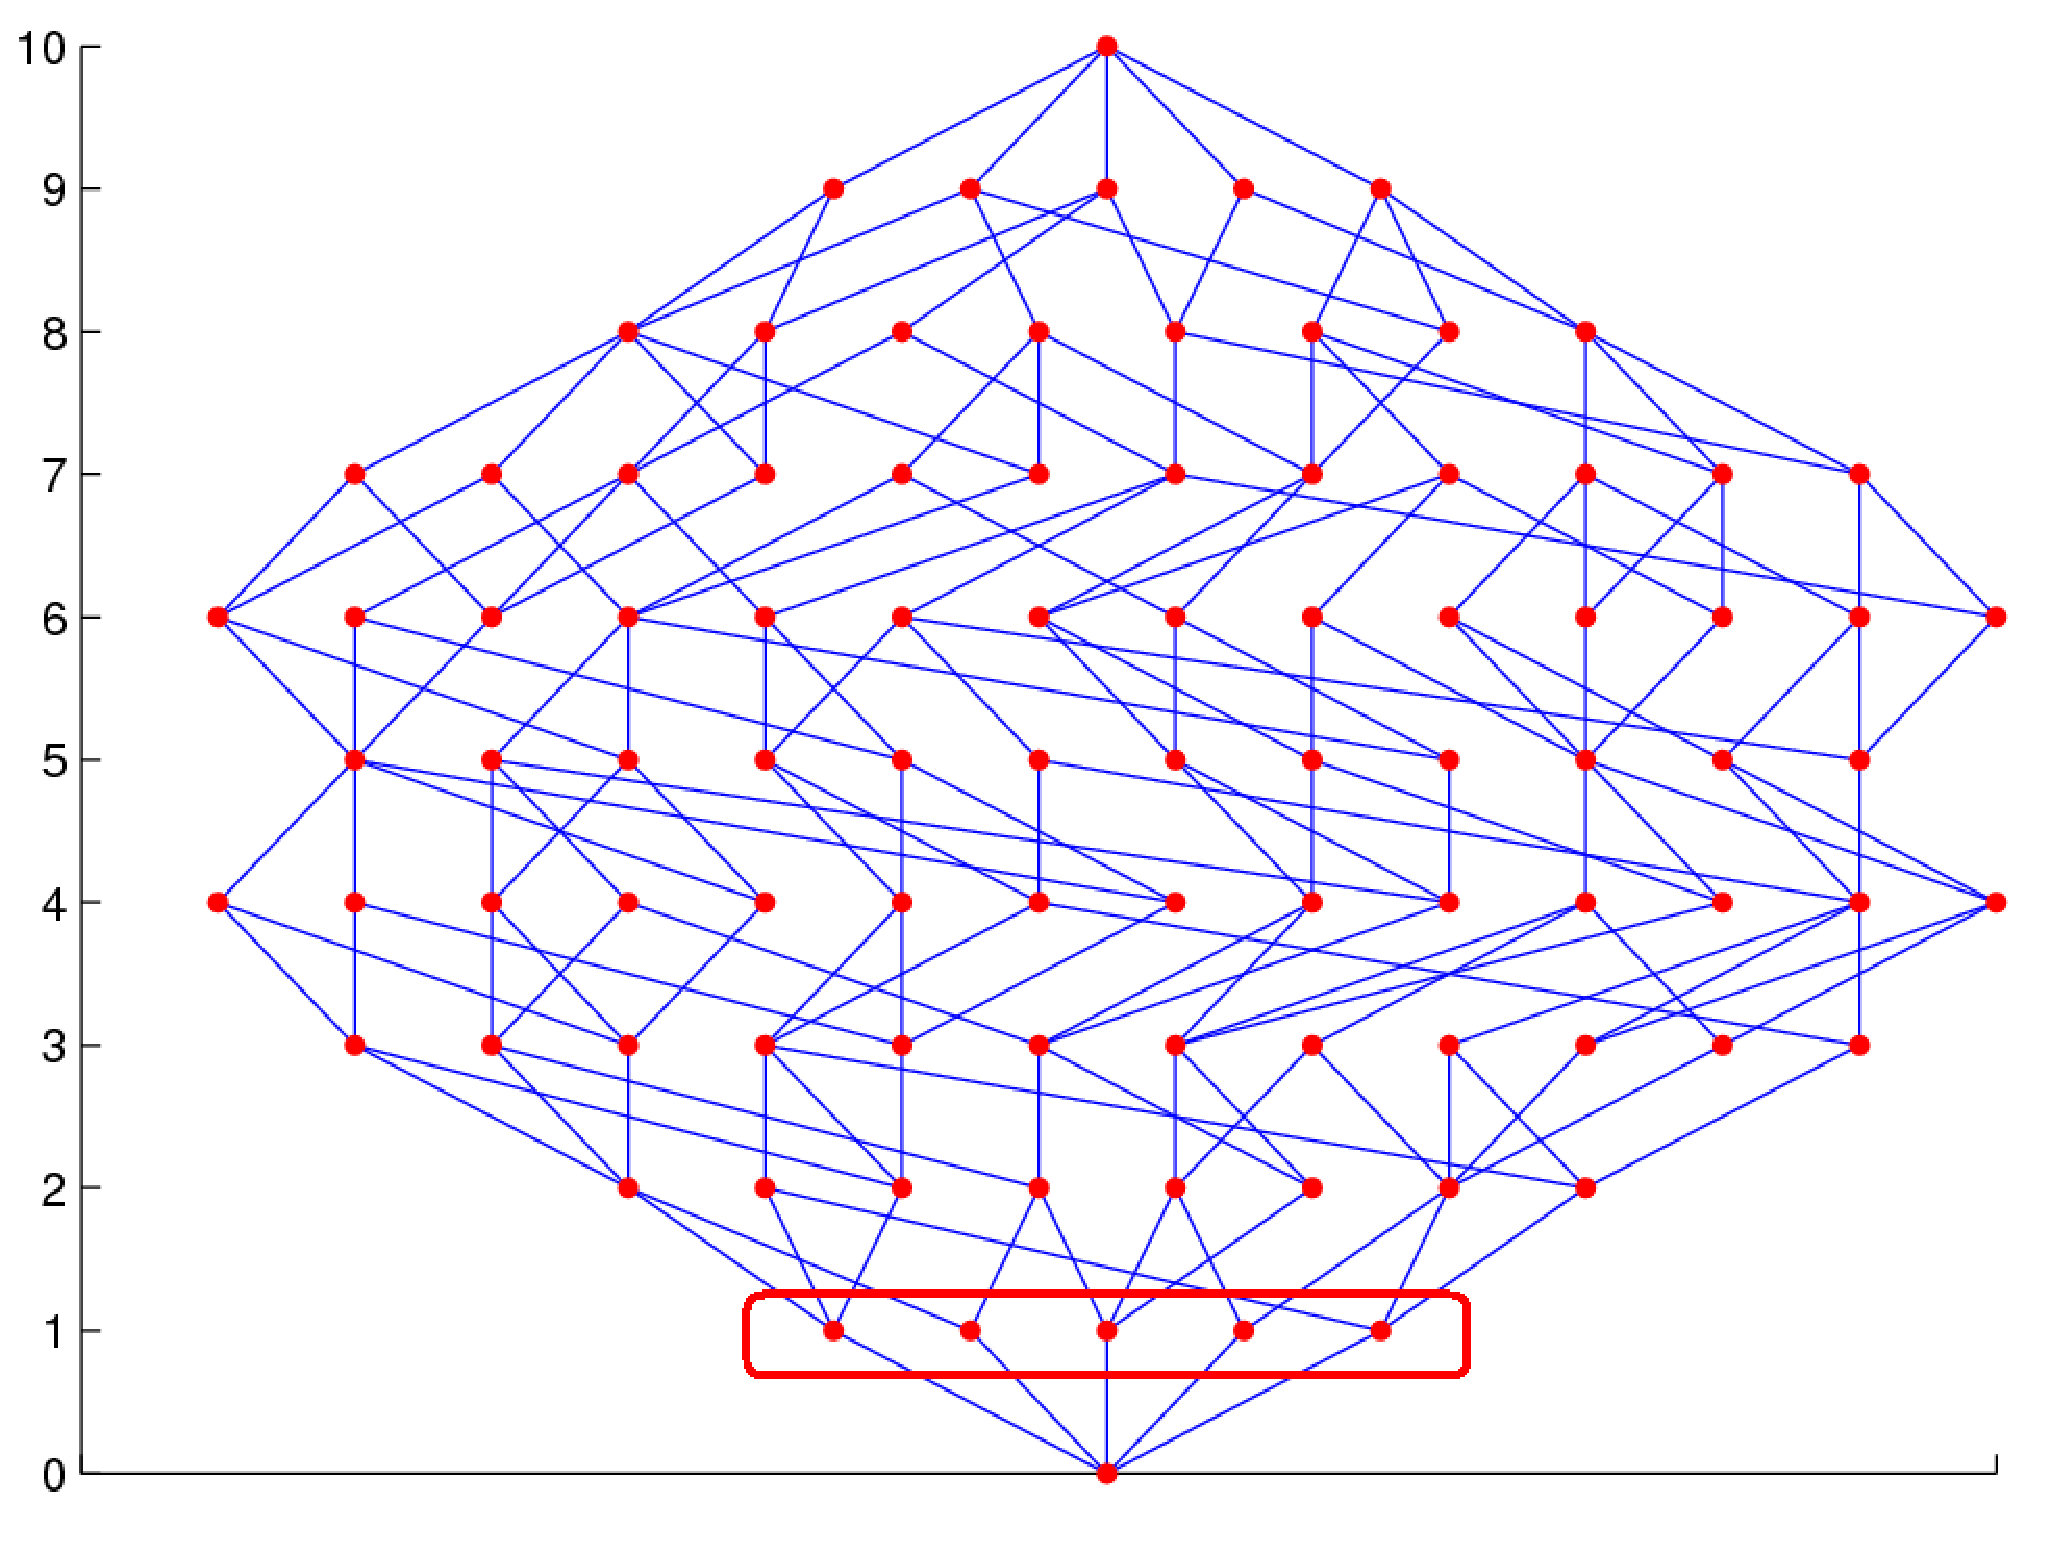
\includegraphics[width = 55mm]{SimpleGraph1.PNG.eps}
    \XYtext(-65mm,43mm){\scriptsize{$m$}}%
    \\\medskip
    \raisebox{-10mm}{(c)}
    \scriptsize
    \begin{tabular}{c|c|ccccc|cccccccc|c}
        & {layer 0} &
        \multicolumn{5}{c|}{layer 1} &
        \multicolumn{8}{c|}{layer 2} \\
        $x_1$ & 0 & 1 & 0 & 0 & 0 & 0 & 1 & 0 & 0 & 0 & 0 & 1 & 1 & 0 & \ldots \\[-0.6ex]
        $x_2$ & 0 & 0 & 1 & 0 & 0 & 0 & 1 & 1 & 0 & 0 & 0 & 0 & 0 & 0 & \ldots \\[-0.6ex]
        $x_3$ & 0 & 0 & 0 & 1 & 0 & 0 & 0 & 1 & 1 & 0 & 0 & 0 & 0 & 1 & \ldots \\[-0.6ex]
        $x_4$ & 0 & 0 & 0 & 0 & 1 & 0 & 0 & 0 & 1 & 1 & 0 & 0 & 0 & 0 & \ldots \\[-0.6ex]
        $x_5$ & 0 & 0 & 0 & 0 & 0 & 1 & 0 & 0 & 0 & 1 & 1 & 1 & 0 & 0 & \ldots \\[-0.6ex]
        $x_6$ & 0 & 0 & 0 & 0 & 0 & 0 & 0 & 0 & 0 & 0 & 1 & 0 & 1 & 0 & \ldots \\[-0.6ex]
        $x_7$ & 0 & 0 & 0 & 0 & 0 & 0 & 0 & 0 & 0 & 0 & 0 & 0 & 0 & 1 & \ldots \\[-0.6ex]
        $x_8$ & 0 & 0 & 0 & 0 & 0 & 0 & 0 & 0 & 0 & 0 & 0 & 0 & 0 & 0 & \ldots \\[-0.6ex]
        $x_9$ & 0 & 0 & 0 & 0 & 0 & 0 & 0 & 0 & 0 & 0 & 0 & 0 & 0 & 0 & \ldots \\[-0.6ex]
     $x_{10}$ & 0 & 0 & 0 & 0 & 0 & 0 & 0 & 0 & 0 & 0 & 0 & 0 & 0 & 0 & \ldots
    \end{tabular}
    \caption{%
        Two-dimensional linearly separable classification task with ${L=10}$ objects of~2~classes
        and 5~linear classifiers that produce exactly one error~(a).
        The~SC-graph over the set of~all \mbox{2-dimensional} linear classifiers~(b).
        The~first layer (${m=1}$) corresponds to 5~classifiers shown at the left chart.
        The~fragment of error matrix corresponding to layers $m=0,1,2$ (c).
    }
    \label{fig:SC-graph-lin}
\end{figure}

SC-graph is much the same as 1-inclusion graph
used in~\cite{haussler94predicting} to obtain lower bounds on VC-dimension.
The VC-dimension may result in~highly overestimated generalization bounds as it is based on the union bound.
In~our combinatorial framework
the SC-graph is~used to~replace the union bound by a~much more accurate technique.

Note that SC-graph can be considered also
as a~subgraph of the Hasse diagram (the graph of transitive reduction)
of~the partial order over error vectors.

\paragraph{SC-bound for pessimistic Empirical Risk Minimization}
\begin{lemma}
\label{lem:pERM}
    If learning algorithm~$\mu$ is pessimistic ERM,
    then conjecture~\ref{hyp:1} holds,
    and for any $a\in A$
    \begin{align*}
        X _a &= \bigl\{ x_{ab}\in\XX \bigm| a\prec b\bigr\}
                \text{~ is the protective subset};\\
        X'_a &= \bigl\{ x\in\XX \bigm| \exists b\in A\colon b\leq a,\; I(b,x)<I(a,x) \bigr\}
                \text{~ is the prohibitive subset}.
    \end{align*}
\end{lemma}
\begin{proof}
    Let us use a proof by contradiction showing that
    if $\mu X = a$, then $X_a\subseteq X$ and $X'_a\subseteq \X$.

    Assume that an~object $x_{ab}\in X_a$ not belonging to~$X$ exists.
    Then ${n(a,X) = n(b,X)}$ because the
    error vectors $a$~and~$b$ differ by exactly one object~$x_{ab}$.
    At~the same time  $n(a,\XX)+1 = n(b,\XX)$,
    therefore the learning algorithm~$\mu$ being pessimistic
    learns the classifier~$b$ rather than~$a$ from the training sample~$X$
    which contradicts the initial condition ${\mu X = a}$.
    Then we conclude that $X_a \subseteq X$.

    Assume that an~object $x\in X'_a$ belonging to~$X$ exists.
    Then ${n(b,X) < n(a,X)}$.
    The learning algorithm~$\mu$ being empirical risk minimizer
    learns the classifier~$b$ rather than~$a$ from the training sample~$X$
    which contradicts the initial condition ${\mu X = a}$.
    Then we conclude that $X'_a \subseteq \X$.
\end{proof}

\begin{corollary}
\label{lem:pERM:corollary}
    Any classifier $a\in A$
    produces errors on all prohibitive objects~$X'_a$ and
    does not produce errors on all protective objects~$X_a$.
\end{corollary}

\emph{Upper connectivity} $q(a)=|X_a|$ of a classifier~$a$
is~the \emph{out-degree} of the vertex~$a$ in the SC-graph,
i.\,e. the number of edges leaving the vertex~$a$.

\medskip
\emph{Lower connectivity} $d(a)=|X'_a|$ of a classifier~$a$
is~the \emph{in-degree}  of the vertex~$a$ in the SC-graph,
i.\,e. the number of edges entering the vertex~$a$.

\medskip
\emph{Inferiority} $r(a)=|X'_a|$ of a~classifier~$a$
is the number of different objects assigned to edges below the vertex~$a$ in the SC-graph.
If~a~correct classifier $a_0\in A$ exists such that $n(a_0)=0$,
then inferiority is equal to the number of~errors, $r(a) = n(a)$.
In~general case, $d(a) \leq r(a)\leq n(a)$.

\begin{theorem}[SC-bound]
\label{th:SC-bound}
    If learning algorithm~$\mu$ is ERM, then for any $\eps\in[0,1]$
    the probability of overfitting is bounded by the weighted sum of FC-bounds over the set~$A$:
    \begin{equation}
    \label{eq:SC-bound}
        Q_\eps(\mu,\XX)
        \leq
        \sum_{a\in A}
            \frac{\CC_{L-q-r}^{\ell-q}}{\CC_{L}^{\ell}}
            \Hyper{L-q-r}{m-r}{\ell-q}{\tfrac\ell L (m - \eps k)},
    \end{equation}
    where
    $q = q(a)$ is upper connectivity,\;
    $r = r(a)$ is~inferiority,\;
    $m = n(a)$ is~the number of errors
    of classifier~$a$ on the general object set~$\XX$.
\end{theorem}
\begin{proof}
    The bound~\eqref{eq:SC-bound} for pessimistic ERM
    follows immediately  from
    theorem~\ref{th:1},
    lemma~\ref{lem:pERM},
    and corollary~\ref{lem:pERM:corollary}.
    Then~\eqref{eq:SC-bound} also holds for any ERM.
\end{proof}

The weight
$P_a = {\CC_{L-q-r}^{\ell-q}} / {\CC_{L}^{\ell}}$
in~the sum~\eqref{eq:SC-bound}
is an upper bound on the probability to~learn the classifier~$a$.
Its~value  decreases exponentially as connectivity~$q(a)$ and inferiority~$r(a)$ increase.
This fact has two important consequences.

First, connected sets of classifiers are less subjected to~overfitting.
Note that an~attempt to use only the fact of~connectedness
with no counting the number of~connections
did not lead to a~tight bound~\cite{sill98phd}.

Second, only a~little part of lower layers contribute significantly to the probability of~overfitting.
This fact encourages effective procedures for level-wise bottom-up SC-bound computation.

The SC-bound~\eqref{eq:SC-bound} is much more tight than the VC-bound~\eqref{eq:VCbound}.
It~can be transformed into the VC-bound by~substituting $q = r = 0$,
i.\,e. by~totally disregarding the SC-graph structure.

%\bibliographystyle{gost71sv}
%\bibliography{MachLearn}

\begin{thebibliography}{1}
\bibitem{haussler94predicting}
    {Haussler~D., Littlestone~N., Warmuth~M.~K.} 
    \emph{Predicting   $\{0,1\}$-functions on randomly drawn points}~// \emph{Inf. Comput.}~---
    \newblock December 1994.~---
    \newblock Vol.~115.~---
    \newblock Pp.~248--292.
\bibitem{sill98phd}
    {Sill~J.}
    \emph{Monotonicity and connectedness in learning systems}: Ph.D. thesis~/ California Institute of Technology.~---
    \newblock 1998.
\bibitem{voron10pria-eng}
    {Vorontsov~K.~V.} 
    \emph{Exact combinatorial bounds on the probability of overfitting for empirical risk minimization}~// 
    {Pattern Recognition and Image Analysis}.~---
    \newblock 2010.~---
    \newblock Vol.~20, no.~3.~---
    \newblock Pp.~269--285.
\end{thebibliography}

\end{document}
